\documentclass[a4paper, 12pt]{article}

\usepackage[top=2cm, bottom=2cm, left=2.5cm, right=2.5cm]{geometry}
\usepackage[utf8]{inputenc}
\usepackage{array}
\usepackage{amsmath}
\usepackage{graphicx}

\graphicspath{{img/}}

\begin{document}
\begin{flushleft}\includegraphics{logo}\\
\textbf{UNIVERSIDADE ESTADUAL DE PONTA GROSSA} \\
SISTEMA UNIVERSIDADE ABERTA DO BRASIL - UAB \\
\underline{Licenciatura em Matemática | Polo UAB em Jacarezinho}\end{flushleft} 
\textbf{ALUNO:} Ricardo Medeiros da Costa Junior   \textbf{RA:} 151774301 \\
\textbf{DISCIPLINA:} Instrumentação para o Ensino de Matemática IV \\
\textbf{ATIVIDADE:} Atividade 10 - Tarefa Descritiva (Valor 9,0)\\ 
\textbf{TUTOR(A):} Giane Correia Silva \\
\textbf{PERÍODO:} Quarto \\\\
\textbf{Atividade - Unidade 3 - Valor 9 pontos  (3 para cada questão)}\\

Escolha \underline{\textbf{3 questões}} de prova de Matemática do ENEM, das aplicadas em 2015, uma questão de cada eixo estruturante. Faça a análise de cada uma delas (veja  exemplo no material obrigatório) conforme os itens descritos abaixo:
\begin{enumerate}
\item Questão 136 \\\\
  Um  estudante  está  pesquisando  o  desenvolvimento de certo tipo de bactéria. Para essa pesquisa, ele utiliza uma  estufa  para  armazenar  as  bactérias.  A  temperatura no  interior  dessa  estufa,  em  graus  Celsius,  é  dada  pela expressão $T(h) = -h^{2}  +  22h - 85 $,  em  que  \emph{h}  representa  as horas do dia. Sabe-se que o número de bactérias é o maior  possível  quando  a  estufa  atinge  sua  temperatura  máxima e, nesse momento, ele deve retirá-las da estufa. A  tabela  associa  intervalos  de  temperatura,  em  graus  Celsius, com as classificações: muito baixa, baixa, média, alta e muito alta. \\\\
  \begin{tabular}{ | c | c | c |}
    \hline
    Intervalos de Temperatura (Graus Celsius) & Classificação \\ \hline
    $ T < 0 $ & Muito baixa \\ \hline
    $ 0 \leq T \leq 17 $ & Baixa \\ \hline
    $ 17 < T < 30 $ & Média \\ \hline
    $ 30 \leq T \leq 43 $ & Alta \\ \hline
    $ T > 43 $ & Muito alta \\ \hline    
  \end{tabular} \\

  Quando o estudante obtém o maior número possível de bactérias, a temperatura no interior da estufa está classificada como:
  \begin{description}
  \item[A] muito baixa.
  \item[B] baixa.
  \item[C] média.
  \item[D] alta.
  \item[E] muito alta.
  \end{description}
  
  \begin{enumerate}
  \item \textbf{Competência: }
    Competência de área 3 - Construir noções de grandezas e medidas para compreensão da realidade e a solução de problemas do cotidiano.
  \item \textbf{Habilidade: }
    H12 - Resolver situação-problema que envolva medidas de grandezas.
  \item \textbf{Eixo Estruturante (PCN+): }
    Álgebra e Funções
  \item \textbf{Interdisciplinaridade: }
    De certa forma sim, pois a questão remete ao aluno refletir sobre alguns organismos estudados na biologia e algumas escalas de temperatura utilizados em física, química e biologia.
  \item \textbf{Contextualização: }
    A questão está contextualizada, pois de acordo com o enunciado fica fácil de entender o que o exercício pede.
  \item \textbf{Grau de dificuldade: }
    Fácil
  \item \textbf{Resolução comentada: }
    Nessa questão é necessário saber qual o máximo da função, para saber em qual intervalo esse máximo se encaixa, para saber quando que as bactérias devem ser removidas do laboratório. Como a função é quadrática e o coeficiente a é maior que zero, é possível determinar o ponto de máximo com coordenada $Xv=\frac{-b}{2a}$ e coordenada $Yv=\frac{-\Delta}{4a}$. Como é apenas a coordenada Y que nos interessa, basta realizar os cálculos:
    $$ \Delta = b^{2}-4ac \Rightarrow $$
    $$ \Delta = 22^{2}-4(-1)(-85) \Rightarrow $$
    $$ \Delta = 484-340 \Rightarrow $$
    $$ \boxed{\Delta = 144} $$\\

    $$Yv = \frac{-\Delta}{4a} \Rightarrow $$
    $$Yv = \frac{-144}{4(-1)} \Rightarrow $$
    $$Yv = \frac{144}{4} \Rightarrow $$
    $$\boxed{Yv = 36} $$\\
  Como 36 está entre 30 e 43, então a temperatura estará \textbf{Alta} quando o estudante obtém o maior número de bactérias. Portanto letra \textbf{D}.
    
  \end{enumerate}
\item Questão 137 \\\\
  A figura representa a vista superior de uma bola de futebol americano, cuja forma é um elipsoide obtido pela rotação de uma  elipse  em  torno  do  eixo  das  abscissas.  Os  valores \emph{a} e \emph{b} são,  respectivamente,  a  metade  do  seu  comprimento horizontal  e  a  metade  do  seu  comprimento  vertical.  Para essa  bola,  a  diferença  entre  os  comprimentos  horizontal e vertical é igual à metade do comprimento vertical.
   \begin{figure}[h!]
   \centering
   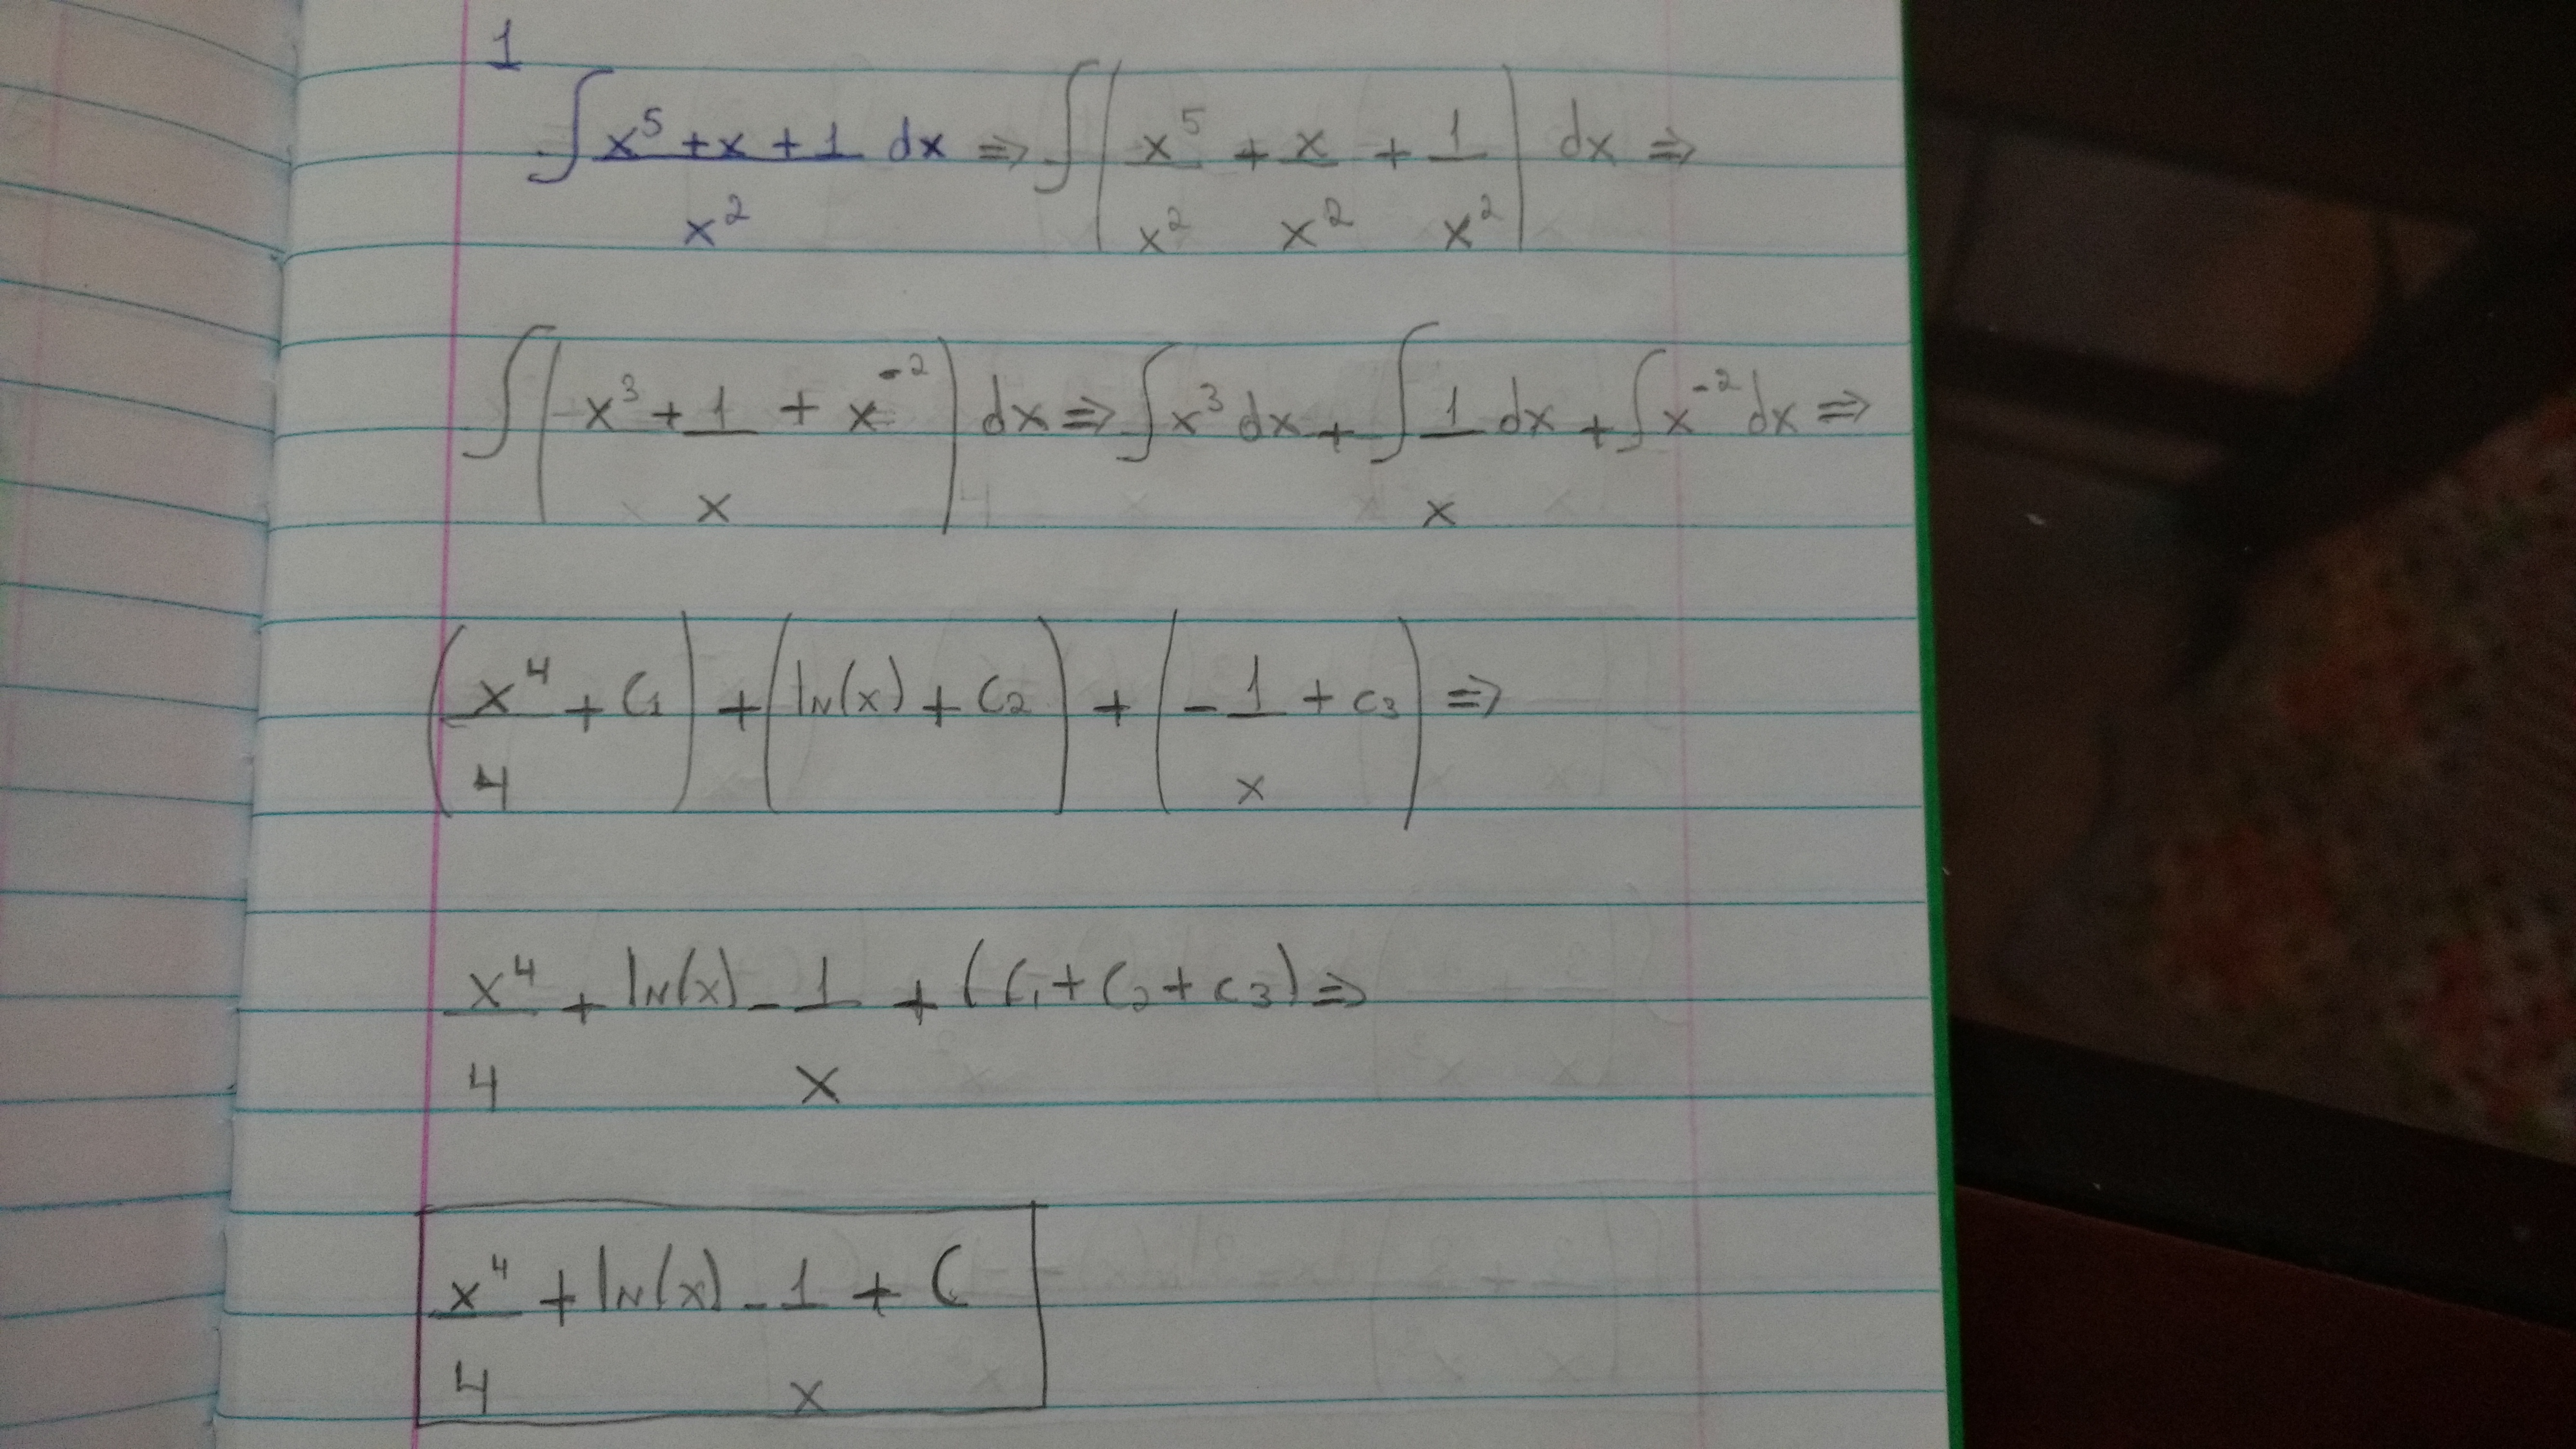
\includegraphics[width=0.3\textwidth]{1}
   \end{figure} \\\\
   Considere que o volume aproximado dessa bola é dado por $ V = 4ab^{2} $.\\
   O volume dessa bola, em função apenas de \emph{b}, é dado por: \\
   \begin{description}
   \item[A] $8b^{3}$
   \item[B] $6b^{3}$
   \item[C] $5b^{3}$
   \item[D] $4b^{3}$
   \item[E] $2b^{3}$     
   \end{description}

  \begin{enumerate}
  \item \textbf{Competência: }
    Competência de área 2 - Utilizar o conhecimento geométrico para realizar a leitura e a representação da realidade e agir sobre ela.
  \item \textbf{Habilidade: }
    H8 - Resolver situação-problema que envolva conhecimentos geométricos de espaço e forma.
  \item \textbf{Eixo Estruturante (PCN+): }
    Geometria.
  \item \textbf{Interdisciplinaridade: }
    Não.
  \item \textbf{Contextualização: }
    Sim, pois explica sobre a bola de futebol americano e o seu formato.
  \item \textbf{Grau de dificuldade: }
    Fácil.
  \item \textbf{Resolução comentada: }
    É dito no enunciado que \emph{a diferença entre os comprimentos horizontal e vertical é igual a metade do comprimento vertical}, ou seja: $2a-2b = b$. Então basta isolar o \textbf{a} e substituir na equação do volume:
    $$2a-2b = b \Rightarrow $$
    $$2a = 3b \Rightarrow $$
    $$a = \frac{3b}{2} $$\\
    
    $$V = 4ab^{2} \Rightarrow $$
    $$V = 4\left(\frac{3b}{2}\right)b^{2} \Rightarrow $$
    $$V = 6b \cdot b^{2} \Rightarrow $$
    $$\boxed{V = 6b^{3}} $$

    Resposta: Letra \textbf{B}
  \end{enumerate}  
\item Questão 138 \\\\
  Após realizar uma pesquisa de mercado, uma operadora de telefonia celular ofereceu aos clientes que utilizavam até 500 ligações no mês o seguinte plano mensal: um valor fixo de R\$12,00 para os clientes que fazem até 100 ligações ao mês. Caso o cliente faça mais de 100 ligações, a partir da 101 até a 300; e caso realizar entre 300 e 500 ligações, será cobra um valor fixo mensagel de R\$32,00.\\
  Com base nos elementos apresentados, o gráfico que melhor representa a relação entre o valor mensal pago nesse plano e o número de ligações feitas é:
   \begin{figure}[h!]
   \centering
   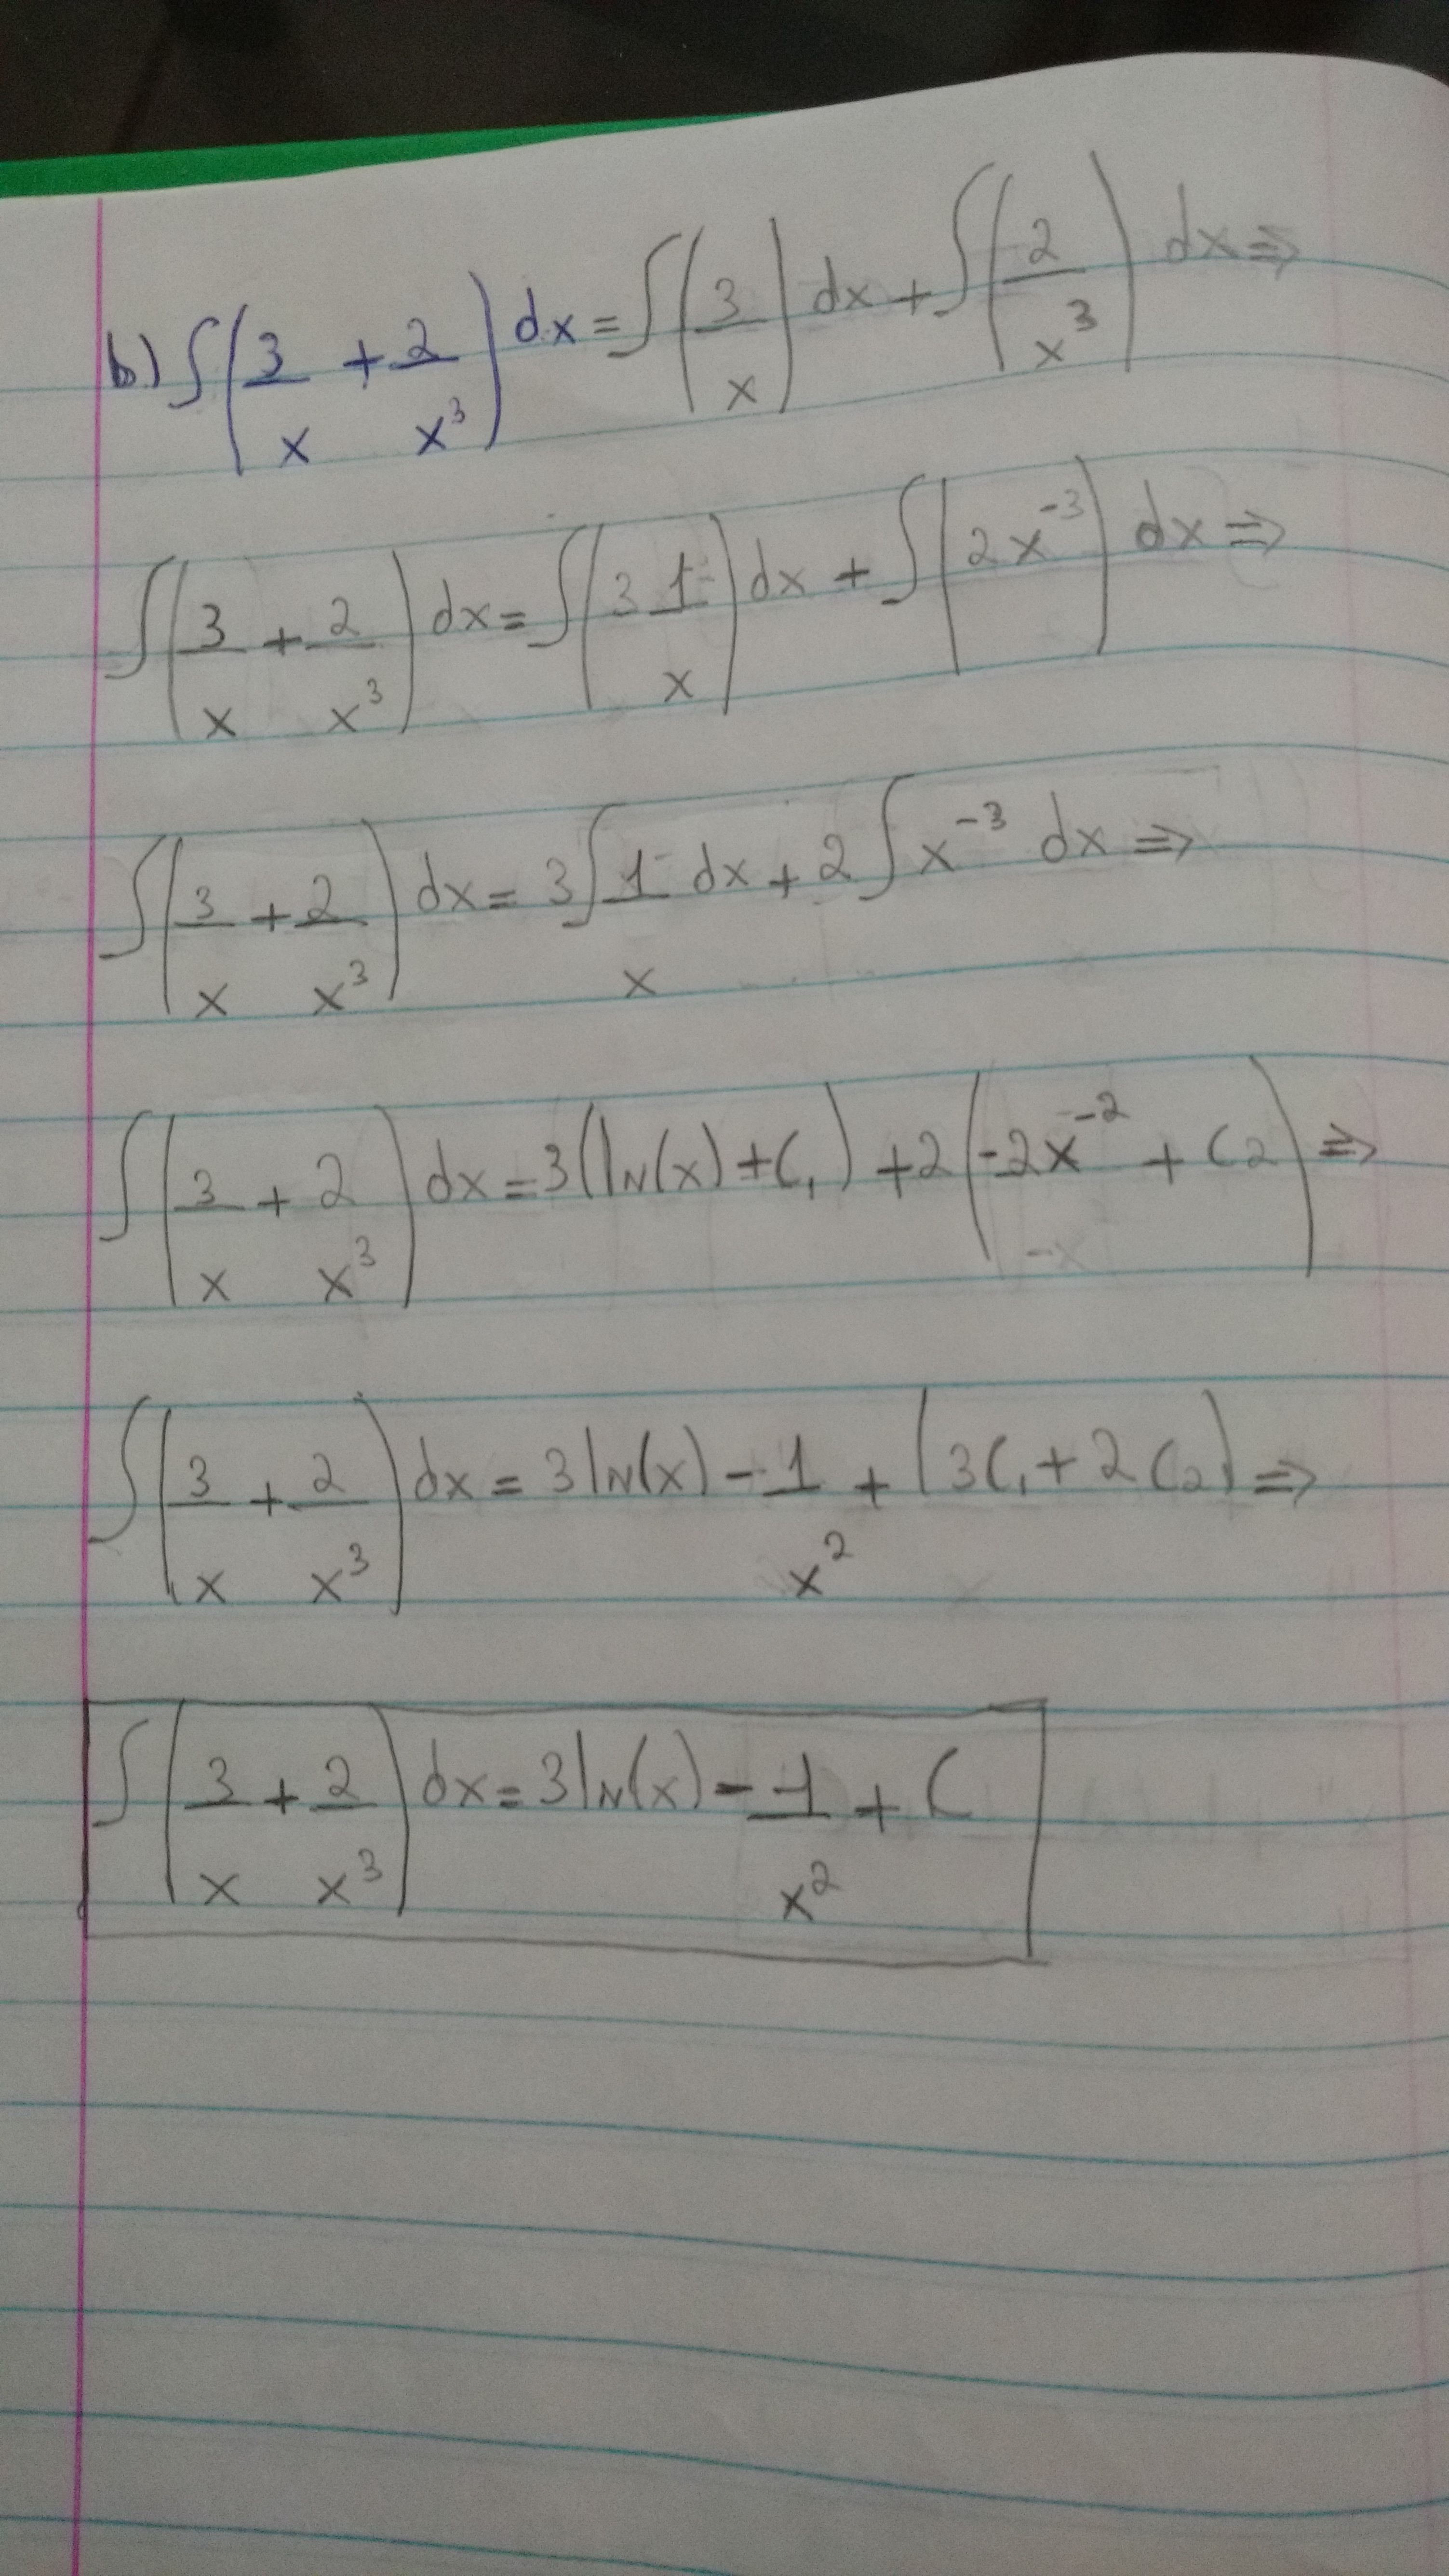
\includegraphics[width=0.3\textwidth]{2}
   \end{figure} \\\\
  
  \begin{enumerate}
  \item \textbf{Competência: }
    Competência de área 6 - Interpretar informações de natureza científica e social obtidas da leitura de gráficos e tabelas, realizando previsão de tendência, extrapolação, interpolação e interpretação.
  \item \textbf{Habilidade: }
    H25 - Resolver problema com dados apresentados em tabelas ou gráficos.
  \item \textbf{Eixo Estruturante (PCN+): }
    Análise de dados.
  \item \textbf{Interdisciplinaridade: }
    Não.
  \item \textbf{Contextualização: }
    Sim, pois a realidade de empresas, gastos e cobrança de tarifas está presente no cotidiano dos alunos.
  \item \textbf{Grau de dificuldade: }
    Fácil.
  \item \textbf{Resolução comentada: }
    O eixo das abscissas representa o número de ligações e o eixo das ordenadas o valor. Como até 100 ligações o preço é fixo, ou seja, constante, até x=100 o y será 12. Depois o preço aumenta de forma proporcional ao número de ligações e após 300 ligações o valor volta assumir o preço constante. Poranto, letra \textbf{B}.
  \end{enumerate}  
\end{enumerate}
\end{document}
